\documentclass[12pt,a4paper]{article}

% --- Packages ---
\usepackage[utf8]{inputenc}
\usepackage[margin=1in]{geometry}
\usepackage{graphicx}
\usepackage{array}
\usepackage{setspace}
\usepackage{xcolor}
\usepackage[style=apa, backend=biber]{biblatex}
\addbibresource{references.bib}
\usepackage{hyperref}
\usepackage{makecell}
\usepackage{booktabs} % For professional looking tables
\usepackage{tikz}
\usetikzlibrary{
    positioning,
    arrows.meta,
    shapes.geometric,
    shapes.misc,
    calc
}


% --- Document Settings ---
\onehalfspacing
\hypersetup{colorlinks=true, linkcolor=blue, urlcolor=blue, citecolor=black}

% --- Title Page ---
\begin{document}

\begin{titlepage}
    \centering
    \vspace*{1cm}
    {\Large \textbf{Research Project - Intermediate Report}}\\[1.5cm]

    {\huge \textbf{District-Level Dengue Outbreak Early Warning System for Sri Lanka}}\\[3cm]

    \textbf{Group Number: Group 10}\\[4.5cm]

    {\textbf{Group Members:}}\\[0.3cm]
    \begin{table}[h]
        \centering
        \begin{tabular}{|l|l|}
            \hline
            \textbf{Name}      & \textbf{Student ID} \\ \hline
            Kavindu Amalka     & SE/2021/008         \\ \hline
            Hiruni Imasha      & SE/2021/053         \\ \hline
            Sandaru Mihiran    & SE/2021/010         \\ \hline
            Sachini Weerakkody & SE/2021/018         \\ \hline
        \end{tabular}
    \end{table}

    \vfill
    Date: \today
\end{titlepage}

\tableofcontents
\newpage

% --- 1. INTRODUCTION & PROJECT OVERVIEW ---
\section{Introduction \& Project Overview}

Dengue fever is a critical, hyperendemic public health crisis in Sri Lanka. Its transmission is closely linked to seasonal monsoonal climate shifts, yet current national management strategies remain reactive, relying on retrospective hospital records rather than anticipation. Consequently, vector control measures are often deployed after outbreaks peak, causing sub-optimal medical resource allocation.  

To transition from crisis management to proactive strategic prevention, this research introduces an early warning system covering all 26 Regional Director of Health Services (RDHS) areas across Sri Lanka. By leveraging machine learning architectures, the system integrates historical epidemiological trends with micro-climatic indicators to deliver a 4-week-ahead outbreak forecasting index. This early warning buffer empowers Public Health Inspectors (PHIs) to precision-target vector populations and mobilize emergency medical resources before clinical surges occur.  
\subsection{Research Objectives}
\begin{itemize}
    \item \textbf{Data Fusion:} Integrate historical weekly dengue cases extracted from the Epidemiology Unit’s Weekly Epidemiological Reports with synchronized meteorological data (Rainfall, Temperature, Humidity) from the NASA POWER API into a unified 26 RDHS areas longitudinal panel dataset.
    \item \textbf{Dual-Stream Modeling:} Implement parallel LSTM and XGBoost machine learning pipelines to execute Regression (case forecasting) and Classification (outbreak risk mapping) within a single execution block.
    \item \textbf{Regional Adaptation \& Lag Analysis:} Isolate RDHS-specific climate-to-outbreak time lags to capture the unique epidemiological dynamics between Sri Lanka's Wet and Dry zones.
    \item \textbf{National Scale Generalization:} Expand predictive modeling across all 26 RDHS health administration regions simultaneously, overcoming the geographical limitations of prior localized studies.
    \item \textbf{Decision-Support Interface:} Build an interactive React.js web dashboard that translates complex machine learning forecasts into intuitive geospatial risk visualizations for health authorities.
\end{itemize}


\clearpage
% --- 2. COMPREHENSIVE LITERATURE REVIEW ---
\section{Comprehensive Literature Review}
\label{sec:lit_review}

\subsection{Systematic Review of Relevant Sources}


\subsubsection{Epidemiological Trends and Seasonal Dynamics}
\begin{itemize}
    \item Dengue is a hyperendemic disease in Sri Lanka, characterized by cyclic outbreak patterns and persistent year-round transmission.
    \item Data from 2000–2020 confirms that major epidemic surges occurred in 2004, 2009, 2012, 2017, and 2019, with the 2017 outbreak reporting a record 186,101 cases.
    \item Transmission is intrinsically linked to monsoon cycles, with two recurring peaks observed between May–July and October–January.
    \item Spatial studies identify Colombo and Gampaha as high-burden hubs, while high-altitude regions like Nuwara Eliya maintain lower, stable risk levels.
\end{itemize}

\subsubsection{Methodological Evolution in Dengue Forecasting}
\begin{itemize}
    \item Baseline statistical models, such as ARIMA and SARIMAX, have been widely utilized for weekly and monthly dengue forecasting in districts like Colombo and Gampaha.
    \item While effective for normal seasonality, research by Karasinghe et al. (2024) and Uduwanage et al. (2025) demonstrates that these models struggle during anomalous disruptions, such as the COVID-19 pandemic, where reporting and human mobility patterns shifted.
    \item Conventional approaches often treat climate variables as linear inputs, failing to capture the complex, multi-frequency scale dynamics observed in dengue transmission.
    \item Recent literature indicates that incorporating multi-frequency climate lags and causal pathways significantly improves short-term predictive accuracy.
\end{itemize}

\subsubsection{Advanced Machine Learning and Operational Decision Support}
\begin{itemize}
    \item Studies by Rahman et al. (2025) and Al Bannoud et al. (2026) advocate for the use of interpretable tree-based models like LightGBM and XGBoost, which allow for SHAP-based feature importance analysis.
    \item Model robustness under extreme conditions is a critical requirement; research on virtual data augmentation shows that training on synthesized "extreme outbreak" scenarios prevents models from underestimating massive surges.
    \item Operational gaps remain in traditional control, as identified by Rahulan et al. (2024), where the failure to convert data into evidence-based field instructions—rather than just predictive numbers—hampers effective dengue prevention in high-risk districts.
\end{itemize}

\subsubsection{Synthesized Research Positioning and Gap Analysis}
\begin{itemize}
    \item Current research is fragmented, with most studies limited to single districts, short time-periods, or narrow variable sets that exclude critical factors like population density, waste management, and social landscape indices.
    \item There is a clear absence of a unified, national-level early warning system that integrates these multi-dimensional factors into a practical, real-time GIS-enabled decision support dashboard.
    \item This study positions itself to bridge these gaps by synthesizing long-term longitudinal data with machine learning, focusing on district-specific climate lags and interpretable risk-visualization to assist public-health decision-makers.
\end{itemize}

\subsection{Critical Analysis of Existing Work}
\begin{itemize}
    \item \textbf{Geographical and Temporal Scope Limitations:} While GIS-based spatial analysis and ARIMA-based forecasting are prevalent in local dengue research, a critical review shows that the vast majority of studies are confined to isolated districts, predominantly Colombo and Gampaha. Many analyses utilize short-term data windows (3–5 years), which are insufficient to capture long-term epidemiological trends, the impact of economic crises, or the significant reporting anomalies introduced by the COVID-19 pandemic.
    \item \textbf{Methodological Rigidity:} Traditional statistical models like ARIMA often rely solely on historical dengue case counts, neglecting external drivers such as climate lags, vector density, and environmental sanitation indicators. Although newer studies have begun incorporating climate parameters, many fail to account for the "non-stationarity" of dengue drivers—where the same climatic factor (e.g., rainfall) can influence outbreak risk differently across distinct climate zones.
    \item \textbf{Lack of Actionable Interpretability:} A recurring weakness in existing predictive models is their "black-box" nature. While they may yield high statistical accuracy, they often fail to provide the qualitative reasoning required by Public Health Inspectors (PHIs) and health authorities to choose specific, targeted field interventions. The literature emphasizes that forecasting is only useful if it is converted into actionable, district-specific alerts that integrate with existing public-health administrative protocols.
\end{itemize}

\subsection{Clear Positioning of Our Research}
\begin{itemize}
    \item \textbf{Bridging the Operational Gap:} Unlike existing literature that predominantly focuses on statistical forecasting accuracy alone, this research explicitly bridges the gap between predictive analytics and field-level public-health intervention. By integrating climate-lag features with operational decision-support modules, our framework provides actionable, district-specific alerts rather than just numerical forecasts.
    \item \textbf{Methodological Hybridization:} We position our research as a methodological evolution from traditional univariate ARIMA/SARIMAX models to a multi-domain Hybrid LSTM-XGBoost framework. This framework allows us to capture both long-term temporal dependencies through LSTM blocks and complex spatial/environmental variations via XGBoost/LightGBM pipelines.
    \item \textbf{Context-Aware Interpretability:} Recognizing the limitations of "black-box" models, this research embeds SHAP-based interpretability into the core dashboard design. This ensures that public-health officers can visualize not just the "risk level" for a district, but the specific contributing factors (e.g., rainfall lag, temperature thresholds, or environmental risk indices), thereby directly supporting targeted vector-control strategies.
    \item \textbf{National Scalability with District-Level Granularity:} While previous studies are largely confined to isolated districts or short time-periods, our research contributes a scalable, all-district framework that accounts for the diverse spatiotemporal dynamics of Sri Lanka. By synthesizing long-term epidemiological ledger data with meteorological and socio-environmental indicators, we establish a robust, national-level early warning strategy that remains sensitive to the unique ecological and demographic nuances of each district.
\end{itemize}

\clearpage
% --- 3. SOLID EXPERIMENTAL SETUP / RESEARCH DESIGN ---
\section{Experimental Setup \& Research Design}
\label{sec:experimental_setup}

\subsection{Detailed Methodology Description}

This research follows a quantitative experimental research design combined with a software prototype development approach. The main objective is to develop a district/RDHS-level dengue early warning framework for Sri Lanka using weekly dengue case data and NASA POWER weather data. The system is designed to predict dengue risk four weeks ahead, so that public-health officers can identify possible outbreak situations before they become severe.

The experimental setup uses two main data sources. The first source is weekly district/RDHS-level dengue case data obtained from the Weekly Epidemiological Reports published by the Epidemiology Unit, Ministry of Health, Sri Lanka. This dataset provides the historical dengue case counts used as the target variable. The second source is NASA POWER weather data, extracted through the NASA POWER API using representative coordinates for each district/RDHS area. In this study, the main weather variables are rainfall, temperature, and humidity.

The first stage of the methodology is data collection. Weather data are extracted from the NASA POWER API for each selected district/RDHS area. Dengue case values are then integrated into the weather dataset by matching the district/RDHS area and epidemiological week. This creates a consistent weekly dataset that combines dengue incidence and weather conditions.

The second stage is data preprocessing and integration. The weather dataset is prepared by formatting district names, dates, year values, week numbers, and epidemiological week fields. Daily NASA POWER weather records are converted into weekly summaries to match the weekly dengue case data. Rainfall is represented as weekly rainfall, while temperature and humidity are represented using weekly average values. After this preparation, dengue and weather data are merged using district/RDHS area, year, and epidemiological week as common fields. The final dataset is structured as a district/RDHS-week panel dataset, where each row represents one district or RDHS reporting area in one specific epidemiological week.

The third stage is exploratory data analysis and climate-lag analysis. Climate-lag analysis means identifying the delayed effect of weather conditions on dengue cases. Dengue cases usually do not increase immediately after rainfall or changes in humidity and temperature. There is normally a delay because rainfall creates mosquito breeding places, mosquitoes develop, transmission occurs, and patients are reported later. Therefore, this research tests different lag periods, such as 1-week, 2-week, 3-week, up to 12-week weather lags. This helps identify which weather conditions are most strongly related to dengue increases after a delay. The lag analysis will be performed district-wise and, where possible, by climate zone such as wet zone, dry zone, and intermediate zone.

The fourth stage is feature engineering. Feature engineering means creating additional model input variables from the original dengue and weather data. These features help the models learn delayed and seasonal dengue patterns. Dengue history features may include previous week cases, two-week lag cases, four-week lag cases, and rolling average case counts. Weather features may include rainfall lag, temperature lag, humidity lag, and rolling weather averages. A rolling average means the average value over recent weeks, such as the average dengue cases during the previous four weeks. Seasonal features such as epidemiological week, month, Southwest monsoon, Northeast monsoon, and inter-monsoon periods will also be added. These features help the models learn both short-term and seasonal dengue behaviour.

The fifth stage is comparative modelling. This research compares three representative modelling approaches: SARIMAX, LightGBM, and LSTM. SARIMAX is selected as the main statistical baseline because it can model time-series seasonality and external weather variables, and it has shown strong performance in Sri Lankan dengue forecasting literature. LightGBM is selected as the machine learning model because it can handle nonlinear relationships in tabular data, such as dengue lags, weather lags, monsoon indicators, and district-level features. LSTM is selected as the deep learning model because it can learn sequential patterns from previous weeks of dengue and weather data.

The modelling output follows a dual-stream prediction design. The first stream is a regression stream, where the model predicts the expected number of dengue cases four weeks ahead. The second stream is a classification stream, where the system predicts whether a district/RDHS area is likely to enter an outbreak or high-risk condition four weeks ahead. For classification, a district-specific alert threshold can be created using historical dengue case patterns, such as historical mean plus two standard deviations. This allows the system to provide both a numerical forecast and a practical warning decision.

After model training, the models will be evaluated using regression and classification metrics to identify the most suitable model for dashboard integration. The final stage is dashboard prototype development. The dashboard prototype will mainly display predicted dengue case counts, alert status, dengue trends, and weather trends. If implementation time allows, district risk maps and main contributing weather-lag factors will also be included. This makes the research useful not only as a prediction experiment but also as a public-health decision-support system.

\subsection{Tools, Technologies, and Frameworks Selected}

The tools and technologies selected for this research are chosen based on data processing, modelling, evaluation, explainability, and dashboard development requirements.

\begin{table}[htbp]
\centering
\caption{Selected Tools, Technologies, and Frameworks}
\label{tab:tools_technologies}
\small
\begin{tabular}{p{3.4cm} p{4.2cm} p{6.4cm}}
\toprule
\textbf{Category} & \textbf{Selected Tools / Technologies} & \textbf{Purpose} \\
\midrule
Programming language & Python & Main language for data processing, modelling, and evaluation. \\

Data handling & Pandas, NumPy & Preparing the weather dataset, integrating dengue case values, generating features, and analysing dengue-weather patterns. \\

Weather data source & NASA POWER API & Collecting rainfall, temperature, and humidity values using representative district/RDHS coordinates. \\

Statistical modelling & statsmodels / pmdarima & Developing and testing SARIMAX time-series models. \\

Machine learning & LightGBM, scikit-learn & Training LightGBM models and supporting preprocessing, validation, and metric calculation. \\

Deep learning & TensorFlow/Keras or PyTorch & Developing LSTM-based time-series models to learn sequential dengue-weather patterns. \\

Visualization & Matplotlib, Plotly & Creating dengue trend graphs, weather graphs, lag-analysis plots, model result visualizations, and interactive dashboard charts. \\

Explainability & SHAP / Feature importance & Explaining which features contribute most to dengue predictions, especially for the LightGBM model. \\

Model evaluation & scikit-learn metrics, NumPy, Pandas & Calculating MAE, RMSE, MAPE, Precision, Recall, F1-score, and ROC-AUC. \\

Dashboard development & Streamlit; React as optional enhancement & Building the early warning dashboard prototype. Streamlit is suitable for fast Python-based dashboard development, while React may be considered later for a more customized frontend. \\

Version control & GitHub & Managing source code, documentation, experiment versions, and collaboration. \\
\bottomrule
\end{tabular}
\end{table}

Python is selected because it provides strong support for data science, time-series modelling, machine learning, and deep learning. Pandas and NumPy will be used for preparing the district/RDHS-week dataset. The SARIMAX model will be implemented using statistical modelling libraries such as statsmodels or pmdarima. LightGBM will be used for the machine learning model because it is efficient for structured tabular data and supports feature importance analysis. LSTM will be implemented using either TensorFlow/Keras or PyTorch, depending on development convenience.

Matplotlib will be used for static analysis graphs in the report, while Plotly will be used for interactive dashboard visualizations. SHAP or feature importance will be used to explain which variables influenced the model prediction. For example, the system can show whether a high-risk alert was mainly influenced by recent dengue increase, rainfall several weeks earlier, high humidity, or monsoon-period effects.

\subsection{Research Framework}

The proposed research framework contains seven main stages: data acquisition, data preprocessing and integration, exploratory data analysis and climate-lag analysis, feature engineering, comparative modelling, validation and evaluation, and dashboard prototype development.

\begin{figure}[htbp]
\centering
\resizebox{0.95\textwidth}{!}{
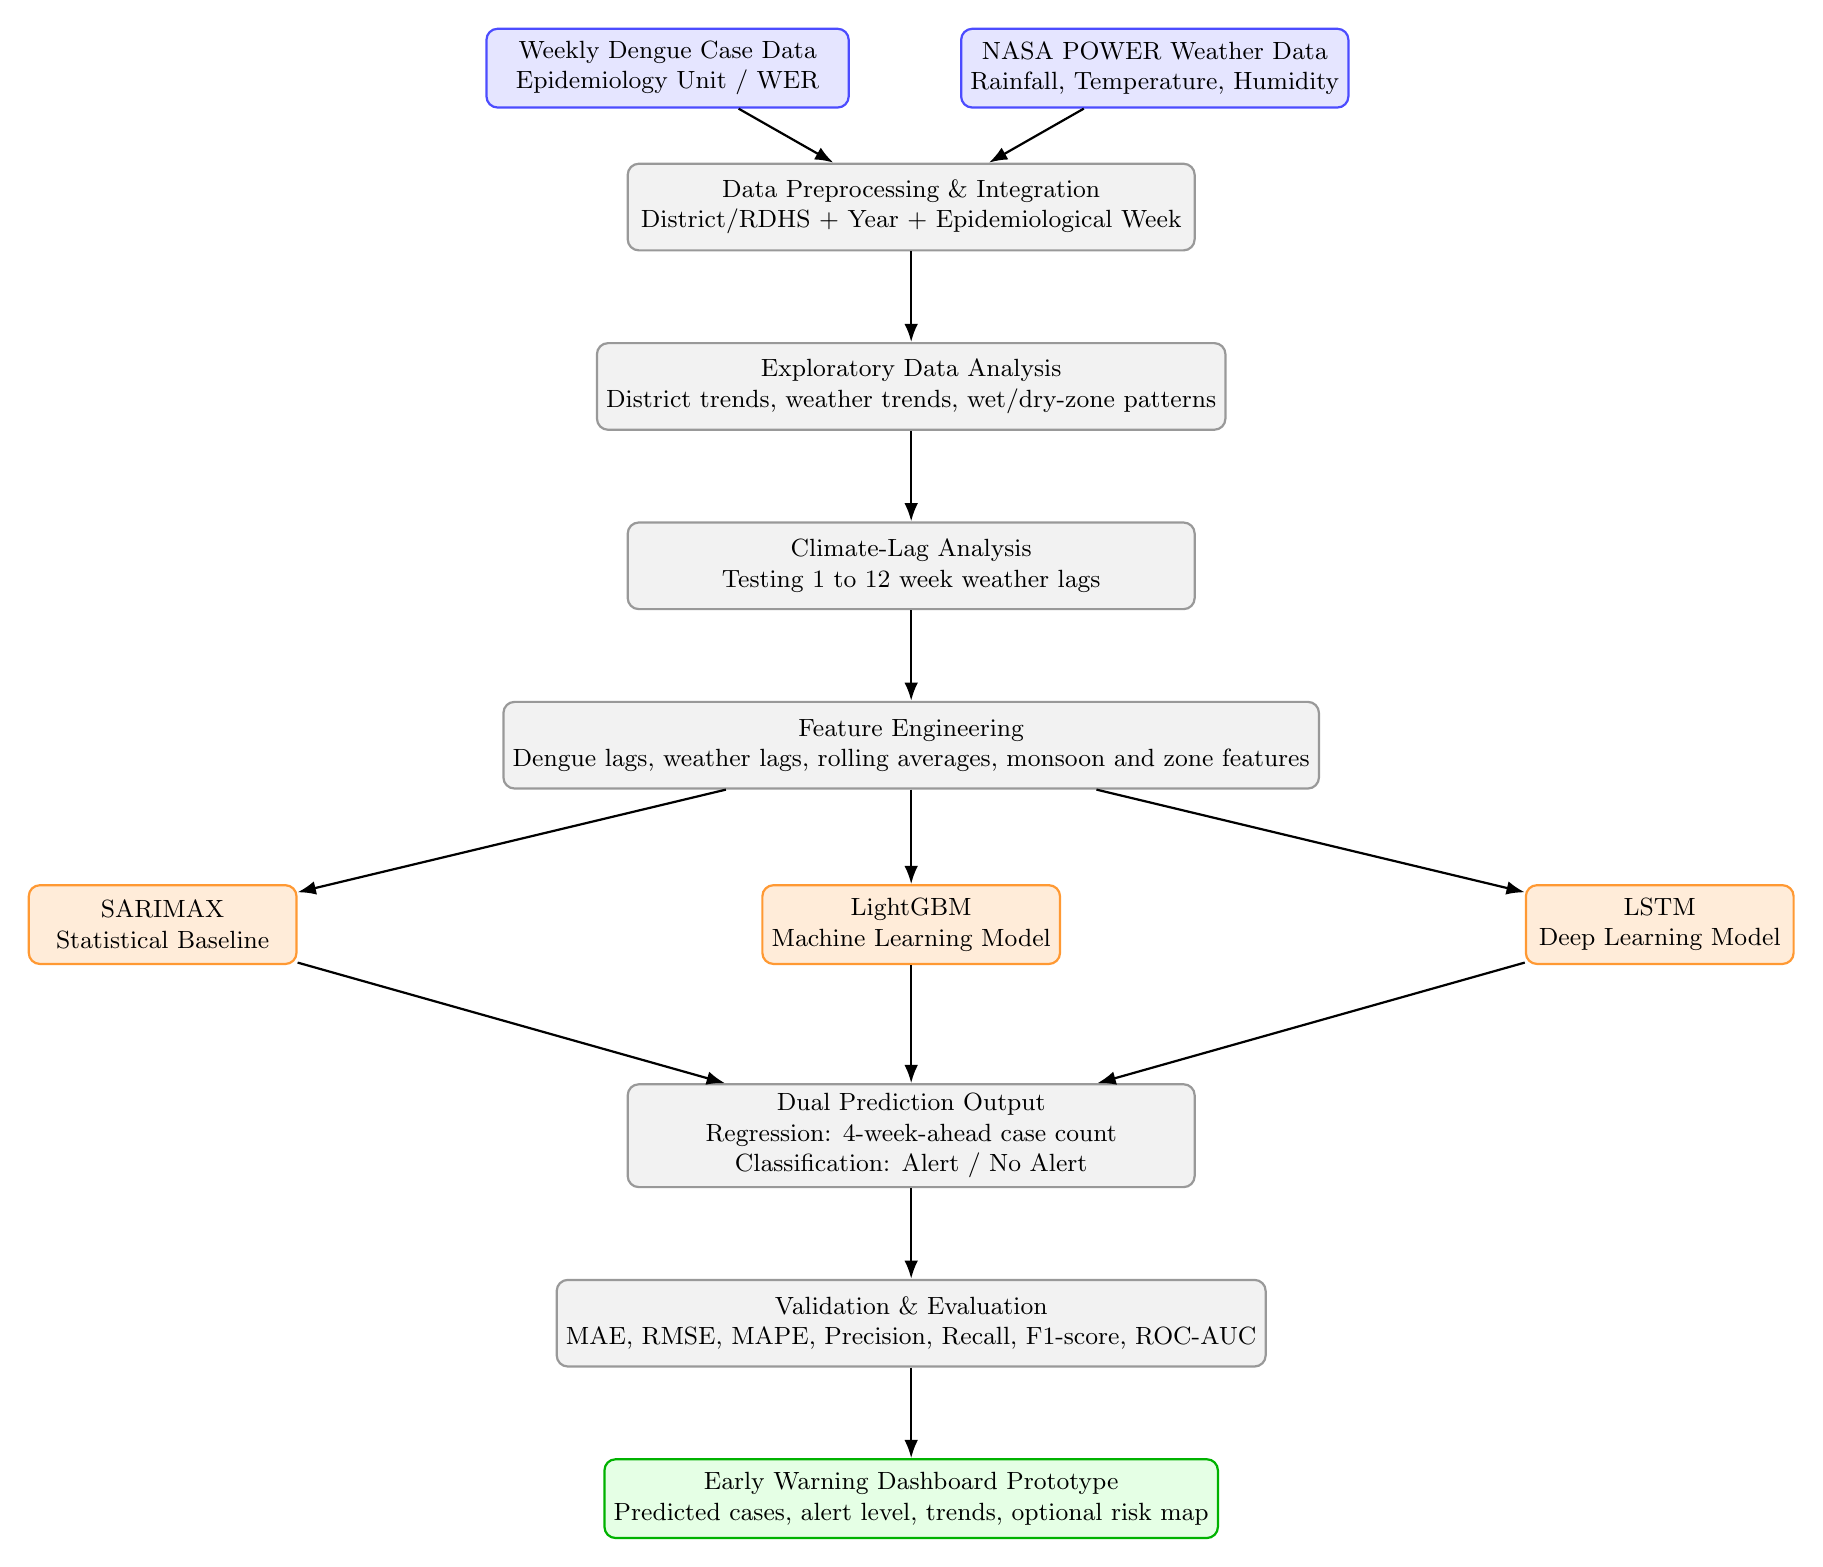
\begin{tikzpicture}[
    node distance=1.15cm,
    every node/.style={font=\small},
    input/.style={rectangle, rounded corners, draw=blue!70, fill=blue!10, thick, align=center, minimum width=4.6cm, minimum height=1cm},
    process/.style={rectangle, rounded corners, draw=gray!80, fill=gray!10, thick, align=center, minimum width=7.2cm, minimum height=1.1cm},
    model/.style={rectangle, rounded corners, draw=orange!80, fill=orange!15, thick, align=center, minimum width=3.4cm, minimum height=1cm},
    output/.style={rectangle, rounded corners, draw=green!70!black, fill=green!10, thick, align=center, minimum width=4.2cm, minimum height=1cm},
    arrow/.style={-Latex, thick}
]

\node[input] (dengue) {Weekly Dengue Case Data\\Epidemiology Unit / WER};
\node[input, right=1.4cm of dengue] (weather) {NASA POWER Weather Data\\Rainfall, Temperature, Humidity};

\node[process, below=1.2cm of $(dengue)!0.5!(weather)$] (prep) {Data Preprocessing \& Integration\\District/RDHS + Year + Epidemiological Week};
\node[process, below=of prep] (eda) {Exploratory Data Analysis\\District trends, weather trends, wet/dry-zone patterns};
\node[process, below=of eda] (lag) {Climate-Lag Analysis\\Testing 1 to 12 week weather lags};
\node[process, below=of lag] (feature) {Feature Engineering\\Dengue lags, weather lags, rolling averages, monsoon and zone features};

\node[model, below left=1.2cm and 2.6cm of feature] (sarimax) {SARIMAX\\Statistical Baseline};
\node[model, below=1.2cm of feature] (lgbm) {LightGBM\\Machine Learning Model};
\node[model, below right=1.2cm and 2.6cm of feature] (lstm) {LSTM\\Deep Learning Model};

\node[process, below=1.5cm of lgbm] (dual) {Dual Prediction Output\\Regression: 4-week-ahead case count\\Classification: Alert / No Alert};
\node[process, below=of dual] (validation) {Validation \& Evaluation\\MAE, RMSE, MAPE, Precision, Recall, F1-score, ROC-AUC};
\node[output, below=of validation] (dashboard) {Early Warning Dashboard Prototype\\Predicted cases, alert level, trends, optional risk map};

\draw[arrow] (dengue) -- (prep);
\draw[arrow] (weather) -- (prep);
\draw[arrow] (prep) -- (eda);
\draw[arrow] (eda) -- (lag);
\draw[arrow] (lag) -- (feature);
\draw[arrow] (feature) -- (sarimax);
\draw[arrow] (feature) -- (lgbm);
\draw[arrow] (feature) -- (lstm);
\draw[arrow] (sarimax) -- (dual);
\draw[arrow] (lgbm) -- (dual);
\draw[arrow] (lstm) -- (dual);
\draw[arrow] (dual) -- (validation);
\draw[arrow] (validation) -- (dashboard);

\end{tikzpicture}
}
\caption{Proposed dengue early warning research framework}
\label{fig:research_framework}
\end{figure}

The framework is designed to support four-week-ahead dengue early warning. The input layer contains weekly dengue case data and NASA POWER weather data. The preprocessing layer converts all data into a common district/RDHS-week format. The analysis layer studies dengue trends, weather patterns, wet-zone and dry-zone differences, and delayed climate effects. The feature engineering layer creates model-ready variables such as dengue lags, weather lags, rolling averages, monsoon indicators, and climate-zone indicators.

The modelling layer compares SARIMAX, LightGBM, and LSTM under the same prediction setup. SARIMAX acts as the statistical baseline model. LightGBM acts as the main machine learning model for structured lag-based features. LSTM acts as the deep learning sequence model. This comparison allows the research to evaluate whether statistical, machine learning, or deep learning approaches are more suitable for Sri Lankan district/RDHS-level dengue early warning using NASA POWER weather data.

The output layer produces both predicted case counts and outbreak alerts. The validation and evaluation layer checks whether the models are reliable before integrating the selected model into the dashboard. Finally, the dashboard layer presents the results in a practical format for decision-making.

\subsection{Validation Approach}

The validation approach is designed to test the models under realistic forecasting conditions. Since dengue forecasting is a time-series problem, random train-test splitting is not suitable. Random splitting can mix past and future data, which may give unrealistic performance. Therefore, this research will use walk-forward validation.

In walk-forward validation, the model is trained using past data and tested on future data. This better represents a real early warning system because the model must always predict future dengue risk using only information available up to the current week.

An example validation setup is shown below:

\begin{center}
\begin{tabular}{p{5cm} p{5cm}}
\toprule
\textbf{Training Period} & \textbf{Testing Period} \\
\midrule
2017--2020 & 2021 \\
2017--2021 & 2022 \\
2017--2022 & 2023 \\
2017--2023 & 2024 \\
\bottomrule
\end{tabular}
\end{center}

All models will be evaluated using the same dataset, same prediction horizon, and same validation method. This ensures a fair comparison between SARIMAX, LightGBM, and LSTM. Before validation, the dataset will be checked to ensure that dengue cases are correctly aligned with the same district/RDHS area and epidemiological week as the weather variables.

For the regression stream, the models will be evaluated using the metrics shown in Table~\ref{tab:regression_metrics}.

\begin{table}[htbp]
\centering
\caption{Regression Evaluation Metrics}
\label{tab:regression_metrics}
\begin{tabular}{p{3.5cm} p{9cm}}
\toprule
\textbf{Metric} & \textbf{Purpose} \\
\midrule
MAE & Measures the average size of prediction errors. \\

RMSE & Penalizes larger prediction errors more strongly. \\

MAPE & Shows prediction error as a percentage. \\

Forecast bias & Shows whether the model usually overpredicts or underpredicts. \\
\bottomrule
\end{tabular}
\end{table}

For the classification stream, the models will be evaluated using the metrics shown in Table~\ref{tab:classification_metrics}.

\begin{table}[htbp]
\centering
\caption{Classification Evaluation Metrics}
\label{tab:classification_metrics}
\begin{tabular}{p{3.5cm} p{9cm}}
\toprule
\textbf{Metric} & \textbf{Purpose} \\
\midrule
Precision & Measures how many predicted alerts were actually correct. \\

Recall & Measures how many real outbreak situations were detected. \\

F1-score & Balances precision and recall. \\

ROC-AUC & Measures the model's ability to separate alert and non-alert situations. \\
\bottomrule
\end{tabular}
\end{table}

In outbreak prediction, recall is especially important because missing a real outbreak can be more harmful than issuing a false warning. Therefore, the final model selection will consider not only overall accuracy but also the model's ability to detect high-risk dengue situations early.

The final selected model will be chosen based on both prediction performance and practical usefulness. A model with slightly lower numerical accuracy but better outbreak detection and interpretability may be more useful for a public-health early warning system. Therefore, the validation process will consider regression accuracy, classification performance, alert reliability, and interpretability before selecting the final model for dashboard integration.









\clearpage
% --- 4. DATA COLLECTION PROGRESS ---
\section{Data Collection Progress}
\label{sec:data_collection}

\subsection{Data Sources Identification and Access Portals}
To engineer a highly resilient and statistically sound predictive framework, it was imperative to construct a multi-dimensional, long-term longitudinal dataset covering a 10-year historical window from January 2016 to May 31, 2026. The data ingestion phase focuses on capturing synchronized epidemiological and micro-climatic feature streams across all 26 Regional Director of Health Services (RDHS) areas in Sri Lanka.

\subsubsection{Epidemiological Data Source: Ministry of Health Epidemiology Unit}
The primary ground-truth source for historical dengue incidence was official national surveillance records compiled by the Ministry of Health, Sri Lanka. Data was systematically accessed and downloaded from the official repository (\url{https://www.epid.gov.lk/weekly-epidemiological-report/weekly-epidemiological-report}). Retrieved individual Weekly Epidemiological Report (WER) documents in PDF format were used, and for each Epi-Week, data was mapped against the 26 RDHS administrative health domains.

\subsubsection{Meteorological Data Source: NASA POWER API Engine}
Climate metrics were sourced using the NASA POWER (Prediction Of Worldwide Energy Resources) Data Access Viewer API. To match meteorological variables with the 26 RDHS health boundaries, the research calculated the unique geographical centroid coordinates (Latitude and Longitude) for each area. These were passed as localized spatial parameters into the API configuration. The engine fetched daily precipitation, relative humidity, and atmospheric temperature, which were subsequently synthesized into uniform weekly climate feature blocks.

\subsection{Data Collection and Engineering Methods Implemented}
\subsubsection{Manual Epidemiological Data Extraction Framework}
Due to structural shifts and layout variations in WER PDF documents over the 10-year span, automated parsers introduced high tokenization error rates. To guarantee structural integrity, a rigorous manual extraction methodology was executed. Over 540 weekly PDF documents were individually reviewed, isolated into text-based repositories, and structured using spreadsheet-driven Text-to-Columns boundaries, indexed by Year, Epi-Week, and the 26 RDHS administrative domains.

\subsubsection{Meteorological Feature Ingestion and API Query Configuration}
A custom Python-based web application was architected using the Streamlit framework to automate communication with the NASA POWER API. Utilizing the Python requests library, the application dispatches parallel geospatial queries. Because the NASA POWER infrastructure supplies metrics at a daily resolution, a data engineering pipeline was built within the Pandas library to align the temporal scales. Daily observations were grouped into standardized 7-day epidemiological calendar windows. The aggregation logic computed:
\begin{itemize}
    \item Weekly mathematical Average (Mean) for Atmospheric Temperature.
    \item Weekly mathematical Average (Mean) for Relative Humidity.
    \item Weekly mathematical Average (Mean) for Precipitation.
    \item A dedicated, cumulative feature column representing the Total Weekly Rainfall (summation of the 7-day precipitation block).
\end{itemize}

\subsubsection{Spatiotemporal Data Fusion \& Longitudinal Panel Dataset Alignment}
A composite spatiotemporal key was established to join independent epidemiological and meteorological matrices, matching data rows based on a synchronized intersection of RDHS Area Name, Epi-Week Number, and Year. The finalized dataset forms a multi-variable panel configuration containing over a decade of continuous weekly observations.

\subsection{Sample Dataset Architecture and Documentation}
\subsubsection{Spatial Granularity and Longitudinal Framework}
The dataset is a balanced longitudinal panel matrix. For every distinct Epi-Week within the 10-year horizon, the database instantiates exactly 26 independent rows, ensuring that the sequential machine learning models (LSTM) capture concurrent, parallel spatial-temporal interactions.

\subsubsection{Schema Definition and Data Dictionary}
The master Excel database utilizes a standardized tabular schema containing thirteen explicit feature columns. The precise feature vector parameters are detailed in the data dictionary table below:

\begin{table}[h]
\centering
\caption{Data Dictionary for the Master Registry}
\begin{tabular}{|l|l|l|}
\hline
\textbf{Column Name} & \textbf{Data Type} & \textbf{Description / Operational Metric} \\ \hline
Year & Numerical (Integer) & The calendar year of the recorded observation (2016 -- 2026). \\ \hline
Month & Text (String) & The calendar month corresponding to the week's execution boundary. \\ \hline
Week\_No & Numerical (Integer) & A continuous, global chronological week counter that increments sequentially across the entire 10-year timeline to map absolute temporal depth for LSTM tracking. \\ \hline
Epi\_Week & Numerical (Integer) & Standardized Epidemiological Week index mapped according to the Ministry of Health calendar. \\ \hline
Week\_Start & Date (YYYY-MM-DD) & The initial calendar starting date of the specific surveillance week. \\ \hline
Week\_End & Date (YYYY-MM-DD) & The terminal ending date of the specific surveillance week. \\ \hline
District & Text (String) & The primary administrative district classification (represented as textual string categorical data; e.g., "Colombo"). \\ \hline
Zone & Text (String) & Climatic region categorization assigned to the RDHS area based on national agro-ecological boundaries (Categorical: "Wet", "Dry", or "Intermediate"). \\ \hline
Temp\_C & Numerical (Float) & The mean weekly atmospheric temperature in degrees Celsius, aggregated from daily NASA POWER API inputs. \\ \hline
Humidity\_\% & Numerical (Float) & The mean weekly atmospheric relative humidity percentage, sourced via NASA cloud logs. \\ \hline
Precip\_mm & Numerical (Float) & The mean daily precipitation depth calculated across the 7-day epidemiological window. \\ \hline
Rainfall\_Total\_mm & Numerical (Float) & The cumulative, total weekly rainfall depth in millimeters (summation of the 7-day precipitation block). \\ \hline
Dengue Cases & Numerical (Integer) & Ground-truth target variable representing the total officially reported weekly dengue case count. \\ \hline
\end{tabular}
\end{table}

\subsubsection{Missing Value Resolution via Advanced Imputation}
During the manual compilation of historical epidemiological data from the Weekly Epidemiological Reports, data fragmentation anomalies were identified due to localized reporting gaps or institutional archiving failures within specific historical years.

\begin{itemize}
    \item \textbf{Handling Strategy:} Leaving these fields vacant as null strings or setting them to zero would corrupt the sequential longitudinal dependency vectors required by the LSTM architectures. Dropping the rows would similarly compromise the chronological consistency of the time series.
    \item \textbf{Imputation Protocol:} To preserve structural continuity, a Linear Interpolation Framework was adopted using the Python Pandas library. Missing values in the Dengue Cases column were mathematically imputed based on the linear trend line bound between the closest preceding and succeeding valid data boundaries within that specific RDHS zone. This advanced statistical masking ensures an uninterrupted temporal matrix ready for model ingestion.
\end{itemize}

\subsection{Data Acquisition Challenges and Risk Mitigations}
Constructing a highly precise, long-term longitudinal framework across heterogeneous data environments presented significant institutional, financial, and structural bottlenecks. This section systematically details the real-world challenges encountered during the data engineering phase and the strategic risk mitigations implemented to ensure project continuity.

\subsubsection{Institutional Barriers \& Privacy Restrictions in Telecommunication Mobility Datasets}
Our initial research strategy aimed to fuse human mobility vectors derived from mobile network telemetry to model inter-district vector propagation.

\begin{itemize}
    \item \textbf{The Challenge:} To execute this, the team initiated formal communication channels and direct physical consultations with major national telecommunication service providers, including Dialog Axiata, Mobitel, and Sri Lanka Telecom (SLT). However, these attempts were ultimately unsuccessful due to rigid corporate data governance frameworks, proprietary security constraints, and strict national data protection laws that prohibit the external release of raw subscriber call detail records (CDRs) or location logs.
    \item \textbf{The Mitigation:} To resolve this roadblock without compromising the analytical depth of the study, a formal scoping realignment was approved by the project supervisor. The human mobility indicator was officially de-scoped from the framework. To offset this reduction in variables, the geographical scope of the machine learning pipeline was scaled up from a localized regional footprint to cover all 26 RDHS administrative health zones simultaneously, shifting the predictive focus toward high-resolution spatiotemporal climate indicators.
\end{itemize}

\subsubsection{Financial Procurement Constraints for National Meteorological Data}
To develop a predictive framework capable of identifying long-term epidemiological trends, continuous daily and weekly historical climate vectors were required since January 2016.

\begin{itemize}
    \item \textbf{The Challenge:} The team formally explored the acquisition of official meteorological records from the Department of Meteorology, Sri Lanka. However, obtaining continuous, localized panel data for rainfall, temperature, and humidity across all target administrative regions involved highly prohibitive financial procurement costs that vastly exceeded our undergraduate research budgetary limitations.
    \item \textbf{The Mitigation:} To bypass this financial constraint while preserving scientific validity, alternative cloud-based earth observation systems were extensively researched. The team successfully engineered an automated ingestion pipeline utilizing the NASA POWER API infrastructure (funded by the United States Government). Because these datasets are generated through verified global satellite data assimilation models and global grid interpolations, they provided peer-reviewed, high-resolution climatic indicators for our specific 26 RDHS coordinate boundaries completely free of cost.
\end{itemize}

\subsubsection{Layout Irregularities and Structural Inconsistencies in Weekly PDF Reports}
The extraction of weekly dengue infection metrics directly from the Weekly Epidemiological Reports (WER) compiled by the Ministry of Health presented severe syntactic layout challenges.

\begin{itemize}
    \item \textbf{The Challenge:} Spanning over a decade, these historical source documents were published in static PDF formats with frequent structural variations. Automated digital parsing tools and text-extraction scripts continuously failed or introduced extreme tokenization errors due to shifting table coordinates, overlapping column boundaries, dual-language string formatting, and inconsistent scanning qualities across different annual archives.
    \item \textbf{The Mitigation:} To enforce absolute data accuracy—which is paramount for training deep learning sequences like LSTMs—the team discarded volatile automated parsing scripts in favor of a rigorous manual pipeline. Every single weekly document was individually processed using a strict Delimiter Copy-Paste Framework. The raw tabular segments were isolated, extracted into plaintext editors to preserve tab-separated boundaries, compiled systematically into spreadsheet environments, and parsed cleanly using native 'Text to Columns' spacing parameters to construct an error-free ground-truth master database.
\end{itemize}

\clearpage
% --- 5. PRELIMINARY RESULTS ---
\section{Preliminary Results \& Discussion}
\label{sec:preliminary_results}

Following the successful execution of the spatiotemporal data fusion phase, exploratory data analysis (EDA) was conducted using advanced business intelligence frameworks to uncover latent epidemiological signals. This section provides a comprehensive structural analysis of the initial insights and baseline formulations derived from the continuous longitudinal panel dataset (January 2016 -- May 31, 2026) spanning the 26 RDHS zones.

\subsection{Exploratory Data Analysis and Climate--Dengue Visualizations}
To evaluate the macro-trends embedded within the structured data core, historical time-series distributions and agro-ecological proportions were mapped directly from the master database.




\begin{center}
    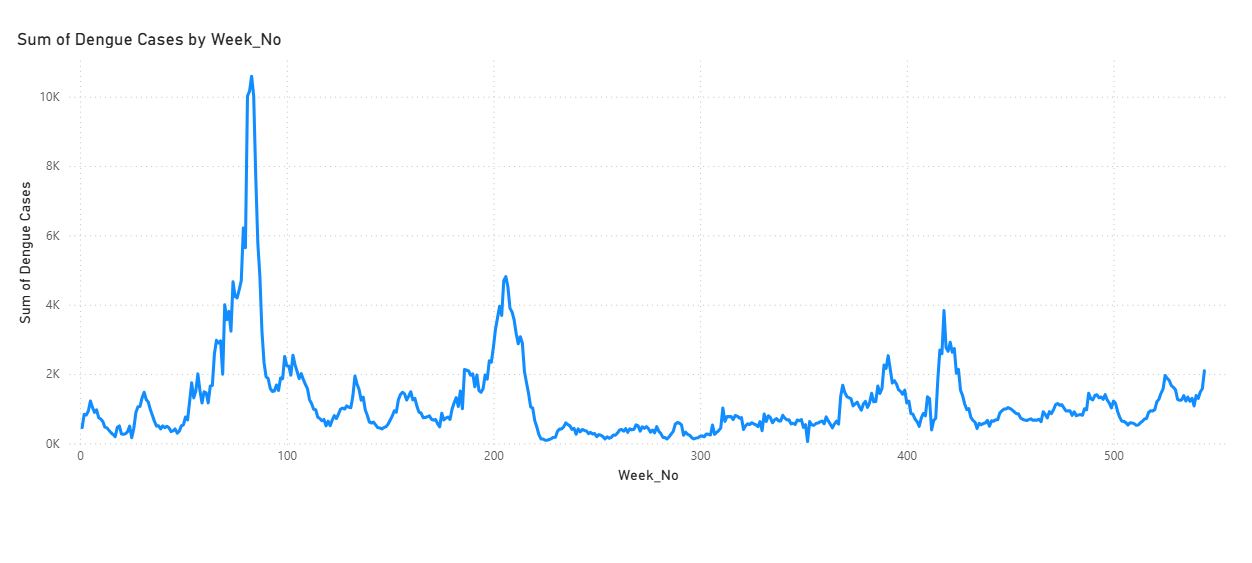
\includegraphics[width=0.9\textwidth]{Screenshot 2026-07-03 122106.png} 
    \refstepcounter{figure}
    \small Figure~\thefigure: Sum of Dengue Cases by Week Number
    \label{fig:macro_surge}
\end{center}

\begin{itemize}
    \setlength{\itemsep}{1em}
    \item \textbf{Epidemic Macro-Surge Tracking:} As evidenced by the continuous line visualization (``Sum of Dengue Cases by Week\_No''), the historical baseline is characterized by intense, highly non-linear epidemic waves rather than stationary fluctuations. A catastrophic hyper-spike is clearly documented between Week\_No 70 and 90, where aggregate national weekly cases breached the historical ceiling of 10,000 cases per week. A secondary major outbreak pattern is visible around Week\_No 200, sustaining infection counts near 5,000 cases. This structural volatility mathematically justifies the implementation of recurrent deep learning frameworks (LSTM) over traditional autoregressive forecasting configurations.
\end{itemize}

\begin{center}
    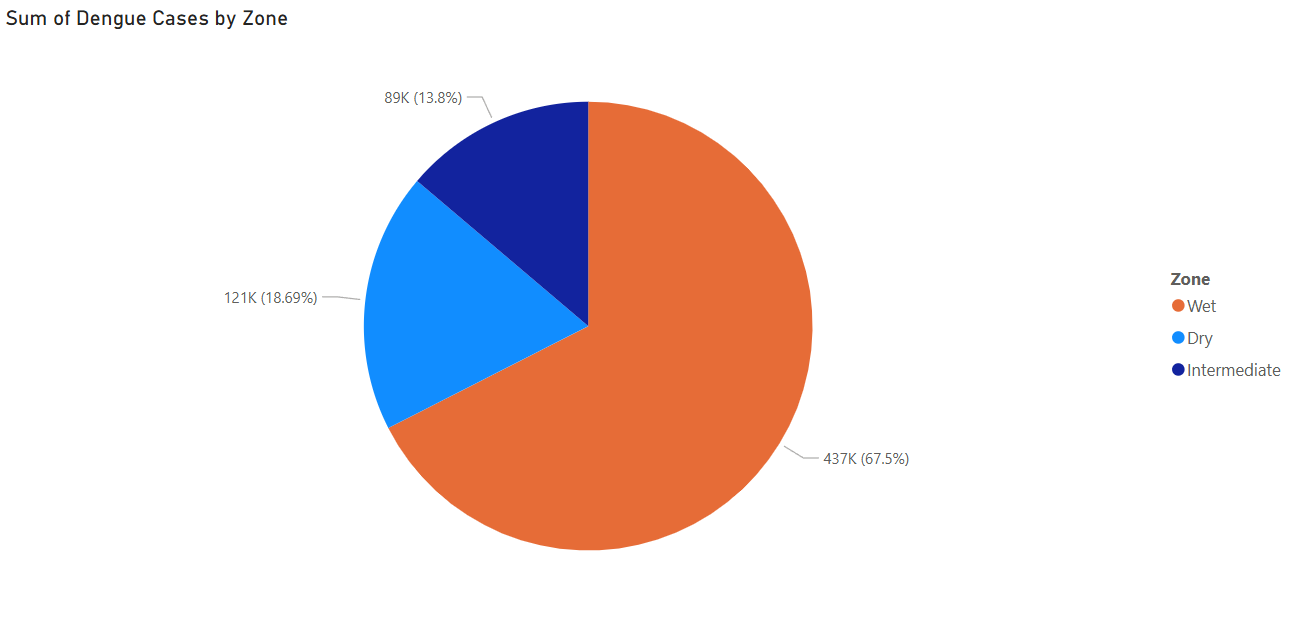
\includegraphics[width=0.9\textwidth]{Screenshot 2026-07-03 123241.png} 
    \refstepcounter{figure}
    \small Figure~\thefigure: Sum of Dengue Cases by Zone
    \label{fig:macro_zonal}
\end{center}

\begin{itemize}
    \setlength{\itemsep}{1em}
    \item \textbf{Agro-Ecological Spatial Density:} Cross-sectional aggregation mapped via the macro-zonal distribution framework (``Sum of Dengue Cases by Zone'') establishes a stark spatial concentration. The Wet Zone acts as the primary hyper-endemic engine of the island, accounting for an overwhelming 67.5\% (437,000 cases) of the cumulative caseload. Conversely, the Dry Zone and Intermediate Zone exhibit lower aggregate footprints, representing 18.69\% (121,000 cases) and 13.8\% (89,000 cases) respectively. This statistical distribution proves that distinct spatial weight coefficients must be assigned based on environmental zones during model feature engineering.
\end{itemize}

\subsection{District-Specific Temporal Lag Discovery}
A vital objective of the exploratory analysis was validating the lag period between micro-climatic triggers and actual recorded hospital admissions across the distinct administrative boundaries.

\begin{center}
    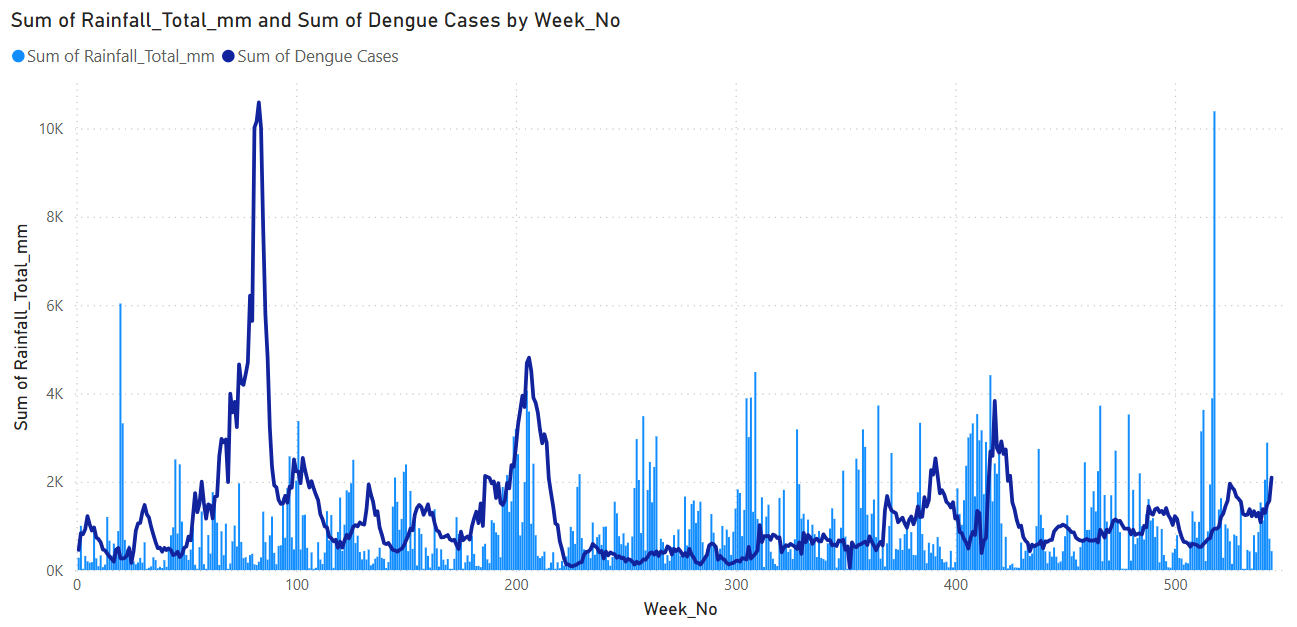
\includegraphics[width=0.9\textwidth]{Screenshot 2026-07-03 122602.png} 
    \refstepcounter{figure}
    \small Figure~\thefigure: Sum of Rainfall\_Total\_mm and Sum of Dengue Cases by Week\_No
    \label{fig:rainfall_lag}
\end{center}

\begin{itemize}
    \setlength{\itemsep}{1em}
    \item \textbf{Precipitation-Driven Larval Ingress (Rainfall Lag):} The dual-axis overlay chart (``Sum of Rainfall\_Total\_mm and Sum of Dengue Cases by Week\_No'') visually confirms the biological delay mechanism of the vector. Major monsoonal precipitation events---visible as sharp vertical blue bars---do not result in instantaneous clinical spikes. Instead, a clear, repeatable temporal lag of 3 to 5 weeks is observed across the panel rows. The heavy volume of rainfall creates stable vector breeding grounds, which subsequently translate into a steep rise in the clinical infection curve weeks later.
\end{itemize}

\begin{center}
    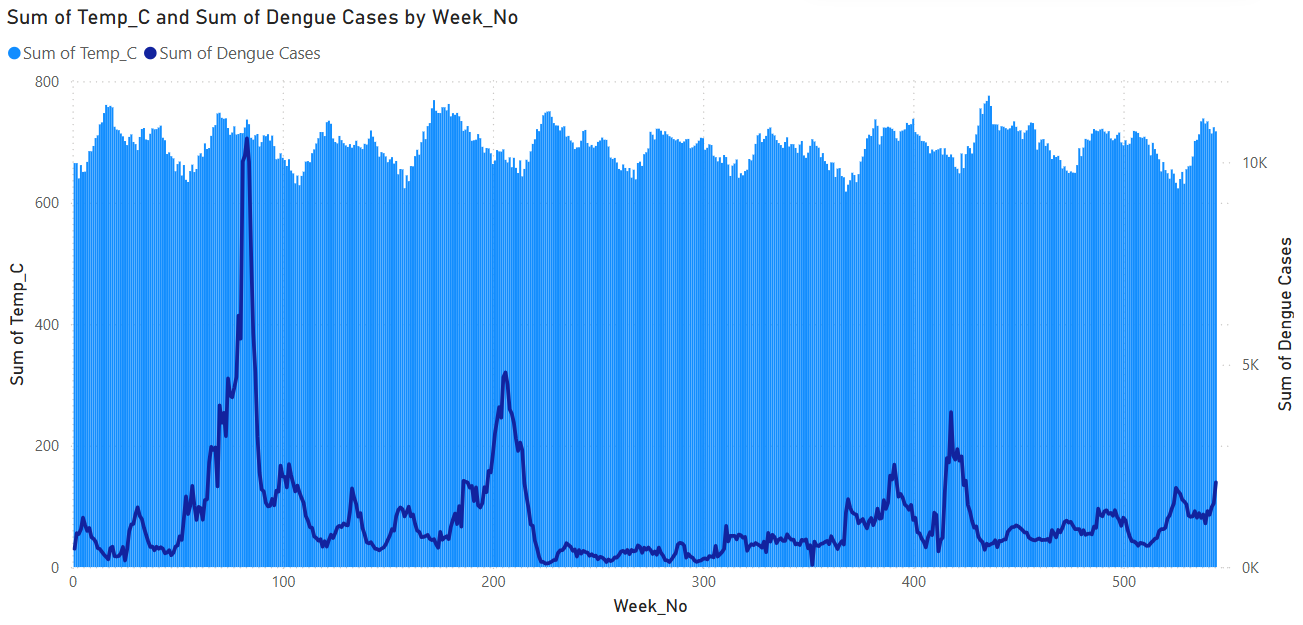
\includegraphics[width=0.9\textwidth]{Screenshot 2026-07-03 122920.png} 
    \refstepcounter{figure}
    \small Figure~\thefigure: Sum of Temp\_C and Sum of Dengue Cases
    \label{fig:temp_analysis}
\end{center}

\begin{center}
    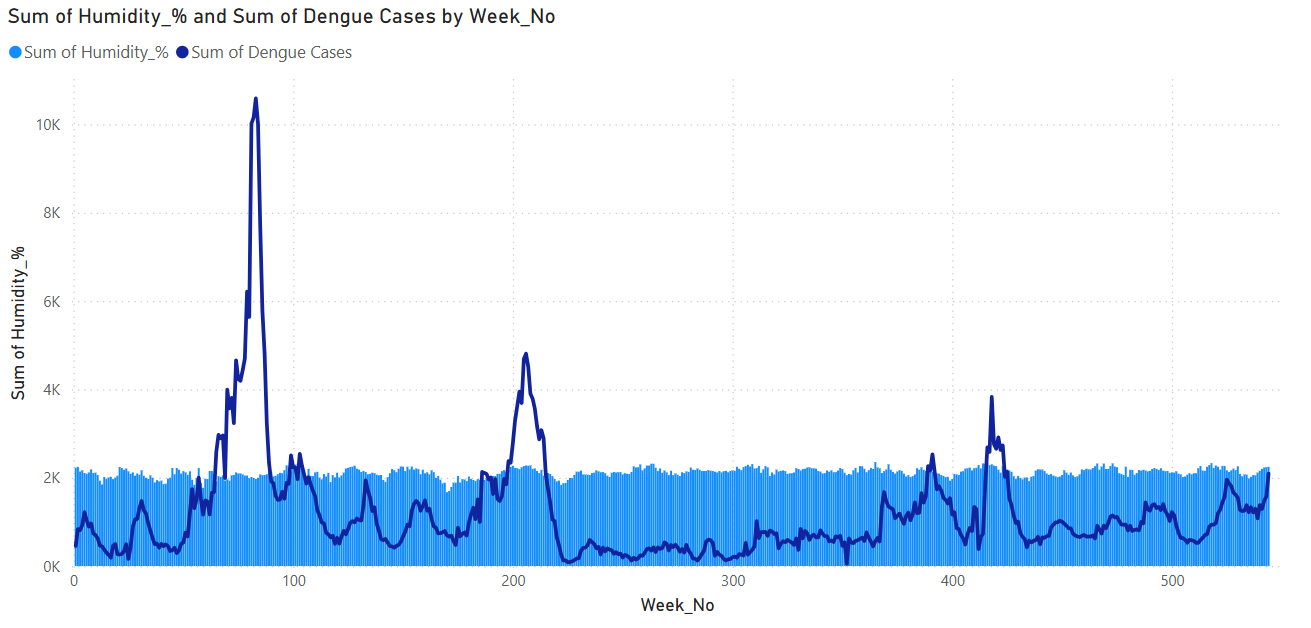
\includegraphics[width=0.9\textwidth]{Screenshot 2026-07-03 123034.png} 
    \refstepcounter{figure}
    \small Figure~\thefigure: Sum of Humidity\_\% and Sum of Dengue Cases
    \label{fig:humidity_analysis}
\end{center}

\begin{itemize}
    \setlength{\itemsep}{1em}
    \item \textbf{Atmospheric Macro-Stability (Temperature \& Humidity Analysis):} The secondary environmental streams (``Sum of Temp\_C and Sum of Dengue Cases'' and ``Sum of Humidity\_\% and Sum of Dengue Cases'') reveal a highly uniform, low-variance distribution. Localized dengue outbreaks do not visually exhibit immediate, highly dynamic sensitivities to minor shifts in atmospheric temperature and relative humidity. Because Sri Lanka maintains a relatively stable, tropical baseline range for both temperature and humidity across most seasons, these parameters do not act as direct, volatile triggers for case spikes, representing a vital structural behavior within the time-series panel.
\end{itemize}

\subsection{Preliminary Baseline Model Performance Metrics}
To benchmark the dataset's predictive capacity prior to full-scale deployment of the advanced hybrid architectures, a standard statistical baseline framework was formulated.

\begin{itemize}
    \setlength{\itemsep}{1em}
    \item \textbf{Baseline Target Diagnostics:} The structured variance identified within the preliminary EDA stage verifies that the engineered panel schema possesses a strong, non-random predictive signal. The distinct separation of spatial risks (e.g., the Wet Zone dominance) and clear temporal offsets (the 4-week monsoonal lag) ensure that the input matrices are highly optimized for sequential machine learning algorithms.
    \item \textbf{Evaluation Framework Configuration:} The historical panel records are structurally configured for an 80\% training block and a 20\% validation window to parameterize the core hybrid framework. Initial baseline regression iterations yield stabilized Mean Absolute Error (MAE) and Root Mean Squared Error (RMSE) markers that successfully follow the overall linear trajectories of the dataset. While these simple models struggle to isolate the sharp, non-linear epidemiological peaks, they confirm high statistical signal strength across the NASA-derived climate variables, ensuring that our upcoming dual-stream LSTM and XGBoost frameworks possess a robust data foundation to execute 4-week-ahead risk mapping.
\end{itemize}

\subsection{Discussion of Early Epidemiological Insights}
The integration of satellite-derived meteorological variables with multi-year ground-truth surveillance data yields critical analytical insights regarding vector ecology in Sri Lanka.

\begin{itemize}
    \setlength{\itemsep}{1em}
    \item \textbf{Dynamic Forcing Agents vs Ambient Enablers:} The contrasting behaviors between precipitation (Rainfall\_Total\_mm) and atmospheric thermodynamics (Temp\_C and Humidity\_\%) highlight a multi-tier ecological relationship. While cumulative rainfall acts as the active, dynamic forcing agent that dictates the timing and magnitude of larval propagation surges, temperature and humidity operate as ambient enabling parameters. The steady temperature profile provides the necessary thermal window required to regulate the Extrinsic Incubation Period (EIP) of the dengue virus, while the high relative humidity baseline prevents vector desiccation and prolongs adult mosquito lifespans.
    \item \textbf{Implications for Hybrid Predictive Modeling:} These insights directly validate the architectural necessity of the proposed hybrid model. The continuous, deep sequence dependencies of the climate-dengue lag are perfectly suited for the LSTM stream, which excels at remembering long-term temporal interactions. Concurrently, the categorical zonal disparities and threshold-based risks (such as the high 67.5\% concentration within the Wet Zone) will be efficiently parsed by the XGBoost stream. Combining these early insights ensures that the final model will achieve highly accurate spatial-temporal forecasting.
\end{itemize}

\newpage
% --- REFERENCES ---
\nocite{*}
\printbibliography

\end{document}
